\documentclass{beamer}
\usetheme{metropolis}
\usepackage{graphicx}
\usepackage{amsmath}
\title{Digital Signal Processing: COSC390}
\author{Jordan Hanson}
\institute{Whittier College Department of Physics and Astronomy}

\begin{document}
\maketitle

\begin{frame}{Course Introduction}
\begin{enumerate}
\item\textit{ \textbf{\alert{What is digital signal processing?}}}
\item \textit{COSC330: Computer Logic and Digital Circuit Design}
\item Read the syllabus for a roadmap
\item \textit{This course can be fast.}
\item \textbf{Data science project and presentation}
\item Textbook: \url{http://dspguide.com}
\item Download and install octave: \url{https://www.gnu.org/software/octave}
\end{enumerate}
\end{frame}

\begin{frame}{Lecture format, with modifications}
\begin{itemize}
\item Theory and examples
\item Programming with Octave
\item Application
\item Study hall
\begin{enumerate}
\item Homework help
\item Project and presentation development
\item Special topics lectures
\end{enumerate}
\end{itemize}
\end{frame}

\begin{frame}{Unit 1.1 Outline}
This lecture will cover:
\begin{enumerate}
\item \alert{Complex numbers 1: Arithmetic and some calculus (continuous and discete) ... see Chapter 30 of text}
\end{enumerate}
Next lectures will cover:
\begin{enumerate}
\item Complex numbers 2: The Fourier series and Fourier transform (continuous and discrete)
\item \textit{Time-permitting}: The Laplace transform (continuous and discrete)
\end{enumerate}
\end{frame}

\section{Complex numbers 1: theory and examples}

\begin{frame}{Complex numbers 1: Definition of a complex number}
A \alert{complex number} is an expression for which one term is proportional to $j = \sqrt{-1}$:
\begin{equation}
z = x + jy
\end{equation}
To call the \textit{complex unit} $j$ is the convention in electrical engineering, and in physics it is often called $i$. \\ \vspace{0.5cm}
Example of complex numbers: $(3+4j)$, $(x_1 + x_2 j)$.  Each number has a \textit{real} part and an \textit{imaginary} part.
\end{frame}

\begin{frame}{Complex numbers 1: Definition of a complex number}
Operations to learn:
\begin{enumerate}
\item Addition
\item Subtraction
\item Real part $\operatorname{Re}$ and $\operatorname{Im}$
\item Multiplication
\item Conjugation
\item Magnitude/Norm
\item Division
\end{enumerate}
Notations to learn:
\begin{enumerate}
\item Cartesian
\item Polar
\item Graphical
\end{enumerate}
\end{frame}

\begin{frame}{Complex numbers 1: Operations}
Addition follows the pattern of two-dimensional vectors:
\begin{align}
z_1 &= 3+4j \\
z_2 &= -2+5j \\
z_1 + z_2 &= 1+9j
\end{align} \\
Subtraction follows the pattern of two-dimensional vectors:
\begin{align}
z_1 &= 3+4j \\
z_2 &= -2+5j \\
z_1 - z_2 &= 5-1j
\end{align}
\end{frame}

\begin{frame}{Complex numbers 1: Operations}
\begin{figure}
\centering
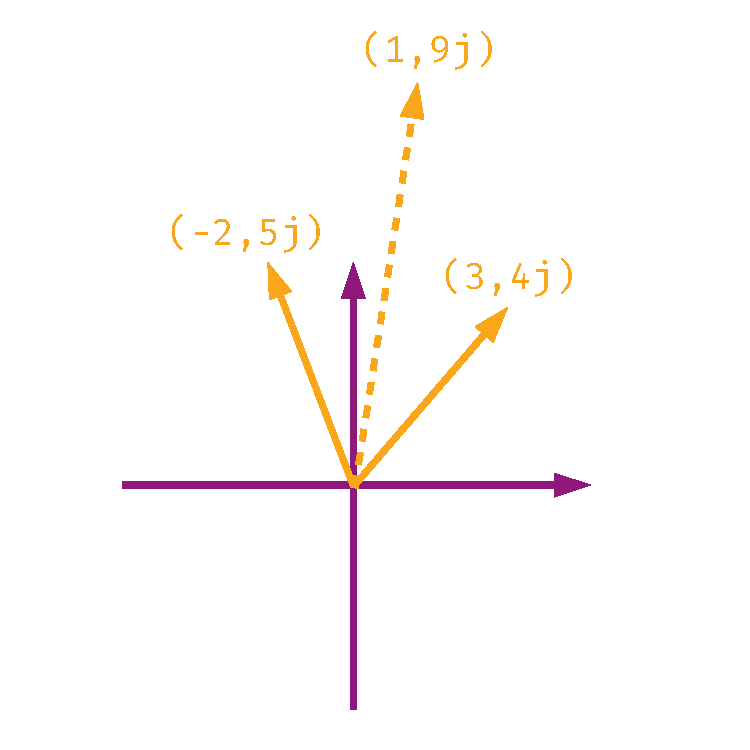
\includegraphics[width=0.45\textwidth]{figures/complexNumbers1.pdf}
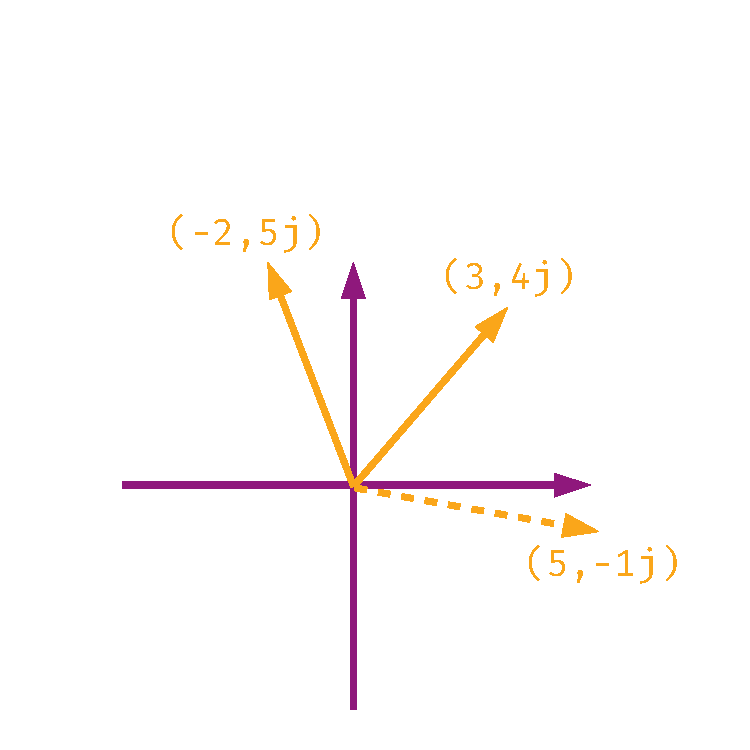
\includegraphics[width=0.45\textwidth]{figures/complexNumbers2.pdf}
\caption{\label{fig:complex1} Complex addition and subtraction follows the pattern of two-dimensional vectors. (Left): Addition of $z_1$ and $z_2$.  (Right): Subtraction of $z_1$ and $z_2$.}
\end{figure}
\end{frame}

\begin{frame}{Complex numbers 1: Operations}
We also have the $\operatorname{Re}$ and $\operatorname{Im}$ operations:
\begin{align}
z_1 &= 3+4j \\
\operatorname{Re}\lbrace z_1 \rbrace &= 3 \\
\operatorname{Im}\lbrace z_2 \rbrace &= 4
\end{align}
These are known as taking the \textit{real}-part and the \textit{imaginary}-part.  The original complex number can be recovered by adding real and imaginary parts together:
\begin{equation}
z_1 = \operatorname{Re}\lbrace z_1 \rbrace + j \operatorname{Im}\lbrace z_1 \rbrace
\end{equation} \\
When we add/subtract complex numbers, we combine the real parts and imaginary parts separately.
\end{frame}

\begin{frame}{Complex numbers 1: Operations}
\textit{Add or subtract, then simplify:}
\begin{enumerate}
\item $z_1 = 7+7j$, $z_2 = -6+3j$.  $z_1+z_2 = $
\item $z_1 = 2+2j$, $z_2 = 3-3j$.  $z_1-z_2 = $
\item $z_1 = 2x+7j$, $z_2 = 2+4xj$.  $z_1+z_2 = $
\end{enumerate}
Let $x=-1$ and $y=1$.  \textit{Evaluate the following expressions:}
\begin{enumerate}
\item $z_1 = x+yj$, $z_2 = y+xj$.  $z_1+z_2 = $
\item $z_1 = x^2+y^2j$, $z_2 = 2y^2+x^2j$.  $z_1-z_2 = $
\end{enumerate}
\end{frame}

\begin{frame}{Complex numbers 1: Operations}
\textit{Multiplication: Recall that $j^2 = -1$.}
\begin{align}
z_1 &= x_1+jy_1 \\
z_2 &= x_2 + j y_2 \\
z_1 \times z_2 &= x_1 x_2 - y_1 y_2 + j (x_1 y_2 + x_2 y_1)
\end{align}
The cross-terms are straightforward, but remember the minus sign when multiplying the imaginary parts.
\end{frame}

\begin{frame}{Complex numbers 1: Operations}
Another similarity with two-dimensional vectors?
\begin{align}
z_1 &= 4-1j \\
z_2 &= 1+4j \\
z_1 \times z_2 &= 8 + 15j \neq 0
\end{align}
What would be the result if we were dealing with regular two-dimensional vectors?
\end{frame}

\begin{frame}{Complex numbers 1: Operations}
\begin{figure}
\centering
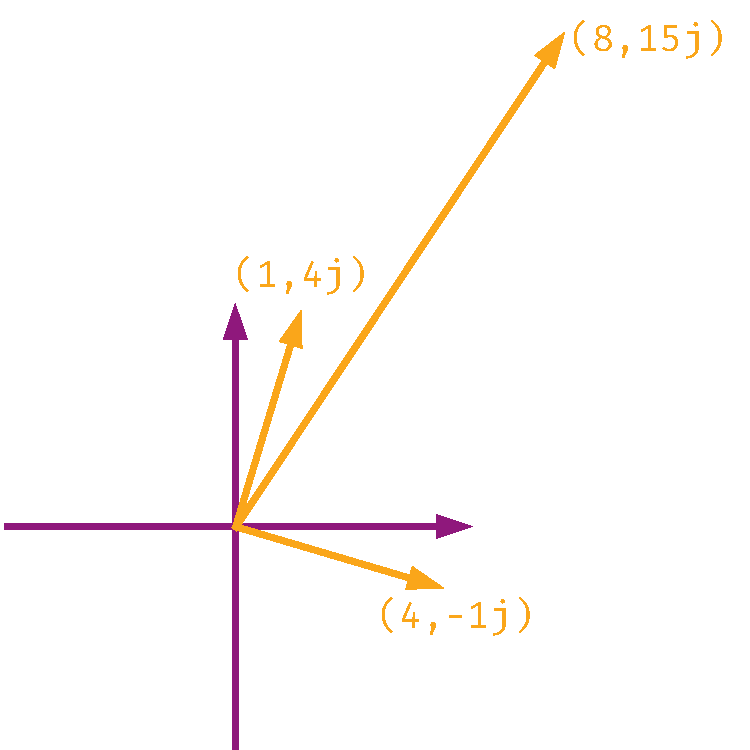
\includegraphics[width=0.45\textwidth]{figures/complexNumbers3.pdf}
\caption{\label{fig:complex2} Complex multiplication resembles the \textit{dot-product} for two-dimensional vectors, with key differences.}
\end{figure}
\end{frame}

\begin{frame}{Complex numbers 1: Operations}
Complex conjugation: change the sign of the imaginary part.
\begin{align}
z_1 &= 4-1j \\
z_1^* &= 4+1j \\
z_2 = &= 2x + 1j \\
z_2^* &= 2x - 1j
\end{align}
Is there a significance to $z_1 z_2^*$?  What about $z_1 z_1^*$?  What about $\sqrt{z_1 z_1^*}$?
\end{frame}

\begin{frame}{Complex numbers 1: Operations}
Let $z = x+jy$.  Compute the following:
\begin{enumerate}
\item $zz^* = $
\item $\sqrt{zz^*} = $
\end{enumerate}
The second item on this list has a special name: the \textit{magnitude} or \textit{norm} of the complex number, $|z|$. \\ \vspace{0.5cm}
Compute the norm of the following complex numbers:
\begin{enumerate}
\item $2+2j$
\item $3+4j$
\end{enumerate}
\end{frame}

\begin{frame}{Complex numbers 1: Operations}
Division of complex numbers: remember that there are multiple steps.
\begin{align}
z_1 &= x_1 + j y_1 \\
z_2 &= x_2 + j y_2 \\
\frac{z_2}{z_1} &= \frac{x_2 + j y_2}{x_1 + j y_1} \\
\frac{z_2}{z_1} &= \frac{z_2 z_1^*}{z_1z_1^*} = \frac{z_2 z_1^*}{|z_1|^2} \\
\frac{z_2}{z_1} &= \frac{\operatorname{Re} \lbrace{z_2 z_1^*}\rbrace}{|z_1|^2} + j \frac{\operatorname{Im} \lbrace{z_2 z_1^*}\rbrace}{|z_1|^2} \\
\frac{z_2}{z_1} &= \frac{x_1 x_2 + y_1 y_2}{x_1^2 + y_1^2} + j \frac{x_1 y_2 - x_2 y_1}{x_1^2 + y_1^2} \label{eq:div}
\end{align}
Using Eq. \ref{eq:div}, show that if $z_1 = z_2$, that $z_2/z_1 = 1$.
\end{frame}

\begin{frame}{Complex numbers 1: Operations}
Evaluate the divisions below:
\begin{enumerate}
\item $z_1 = 1+4j$, $z_2 = 2-2j$.  $z_2/z_1 = $
\item $z_1 = 1+1j$, $z_2 = -3-3j$.  $z_2/z_1 = $
\end{enumerate}
\end{frame}

\begin{frame}{Complex numbers 1: Polar Notation}
\begin{figure}
\centering
\includegraphics[width=0.5\textwidth,angle=270,trim=4cm 2cm 0cm 0cm]{figures/polar.eps}
\caption{\label{fig:complex3} Polar coordinate systems rely on $(\rho,\phi)$ notation, rather than $(x,y)$ notation.}
\end{figure}
\end{frame}

\begin{frame}{Complex numbers 1: Polar Notation}
Polar notation for complex numbers: let $z = x+jy$.
\begin{align}
z &= r \exp(j\phi) \\
r &= |z| = \sqrt{x^2 + y^2} \\
\phi &= \tan^{-1}(y/x)
\end{align}
Useful for multiplication and division:
\begin{align}
z_1 &= r_1 \exp(j\phi_1) \\
z_2 &= r_2 \exp(j\phi_2) \\
z_1 \times z_2 &= r_1 r_2 \exp(j(\phi_1 + \phi_2)) \\
\frac{r_2}{r_1} &= \frac{r_2}{r_1} \exp(j(\phi_2 - \phi_1))
\end{align}
\end{frame}

\begin{frame}{Complex numbers 1: Polar Notation}
\small
Convert these complex numbers from Cartesian to polar form:
\begin{enumerate}
\item $z_1 = 5+13j$
\item $z_2 = 7-24j$
\item $z_3 = 20-21j$
\end{enumerate}
Divide:
\begin{enumerate}
\item $z_3/z_2$
\item $z_3/z_1$
\end{enumerate}
Multiply:
\begin{enumerate}
\item $z_1 \times z_2$
\item $z_1 \times z_1^*$
\end{enumerate}
\end{frame}

\begin{frame}{Complex numbers 1: Polar Notation}
Notice that the procedure for finding the modulus is evident in polar notation:
\begin{equation}
\sqrt{z_1 z_1^*} = \sqrt{r_1 r_1} \exp(j(\phi_1 - \phi_1)/2) = r_1
\end{equation}
Shouldn't we be saying $\pm r_1$?  How does the square root function work in the complex plane?\footnote{Complex fractional-power functions are outside the scope of the course, as it turns out.}
\end{frame}

\begin{frame}{Complex numbers 1: The complex plane}
\begin{figure}
\centering
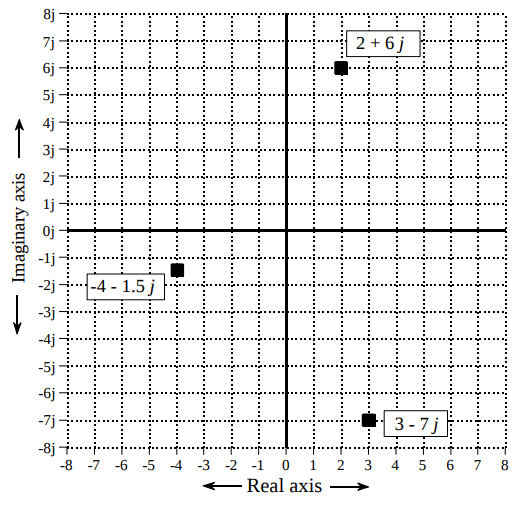
\includegraphics[width=0.5\textwidth]{figures/plane1.png}
\caption{\label{fig:complex4} The real and imaginary axes are an \textit{extension} of the real number line, allowing a broader representation of physical systems than just real numbers.  A prime example is AC circuits.}
\end{figure}
\end{frame}

\begin{frame}{Complex numbers 1: The complex plane}
\begin{figure}
\centering
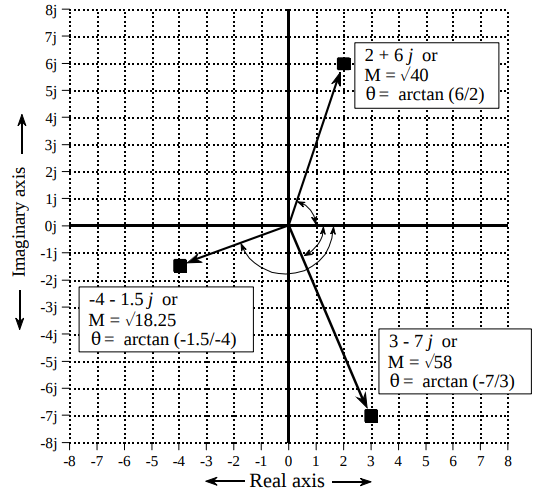
\includegraphics[width=0.5\textwidth]{figures/plane2.png}
\caption{\label{fig:complex5} Consider the complex plane in light of trigonometry.  Think of the magnitude of a complex number as the hypoteneuse of a right triangle.  Then, $\operatorname{Re}\lbrace z \rbrace = |z|\cos\phi$, and $\operatorname{Im}\lbrace z \rbrace = |z|\sin\phi$, and $r = |z| = \sqrt{x^2+y^2}$.}
\end{figure}
\end{frame}

\begin{frame}{Complex numbers 1: The complex plane}
\small
In the trigonometric picture:
\begin{equation}
z = |z| \cos\phi + j |z| \sin\phi
\end{equation}
Proof of polar-notation relationship:
\begin{align}
\exp(j\phi) &= \sum_{i=0}^{\infty} \frac{(j\phi)^n}{n!} = \sum_{i=0}^{\infty} \frac{j^n\phi^n}{n!} \\
\exp(j\phi) &= \sum_{even}^{\infty} \frac{j^n\phi^n}{n!} + \sum_{odd}^{\infty} \frac{j^n\phi^n}{n!} \\
\exp(j\phi) &= \sum_{i=0}^{\infty} (-1)^n \frac{\phi^{2n}}{n!} + j\sum_{i=0}^{\infty} \frac{\phi^{2n+1}}{n!} \\
\exp(j\phi) &= \cos\phi + j\sin\phi \\
|z|\exp(j\phi) &= |z| \cos\phi + j |z| \sin\phi = z
\end{align}
\end{frame}

\begin{frame}{Complex numbers 1: The complex plane}
Thus we have proven:
\begin{equation}
\boxed{ z = x+jy = r \exp(i\phi)
}
\end{equation}
Corollary (prove these):
\begin{align}
\cos(x) &= \frac{1}{2}\left(e^{ix} + e^{-ix}\right) \\
\sin(x) &= \frac{1}{2i}\left(e^{ix} - e^{-ix}\right)
\end{align}
Suppose we have now have a voltage signal
\begin{equation}
v_i(t) = A_i \cos(2\pi f_i t + \phi_i)
\end{equation}
We may write
\begin{equation}
v_i(t) = A_i \operatorname{Re}\lbrace \exp(j(2\pi f_i t + \phi_i)) \rbrace
\end{equation}
\end{frame}

\begin{frame}{Complex numbers 1: The complex plane}
What if we treat the signal as complex, but agree to take the real part at the end of our calculations?
\begin{equation}
v_i(t) \rightarrow A_i \exp(j(2\pi f_i t + \phi_i))
\end{equation}
As long as we take the real part of the right hand side, we'll have the original signal. \\ \vspace{0.5cm}
Now contemplate the addition of signals of the same frequency, but different amplitudes and phases.  Let $x_i = 2\pi ft+\phi_i$.  A signal comprised of $N$ sinusoids can be written
\begin{equation}
V_i(t) \rightarrow \sum_i^N a_i \exp(jx_i)
\end{equation}
\end{frame}

\begin{frame}{Complex numbers 1: The complex plane}
Remember that $x_i = 2\pi ft+\phi_i$.  The sum of two sinusoids in the complex plane can then be written\footnote{Notice that taking the real part distributes if the original signal is real.}
\begin{equation}
V(t) = a_1\exp(x_1) + a_2\exp(x_2)
\end{equation}
\begin{enumerate}
\item Compute $|V|^2 = V^*V$, and $\phi_2 - \phi_1 = \pi$, $\phi_2 - \phi_1 = 0$.
\item What is $\phi_V = \tan^{-1}(\operatorname{Im}\lbrace V \rbrace/\operatorname{Re}\lbrace V \rbrace)$ in each case?
\end{enumerate}
Why do these results make sense?  Thus, the complex numbers encapsulate the concepts of \textit{constructive} and \textit{destructive} interference.
\end{frame}

\begin{frame}{Complex numbers 1: The complex plane}
\small
What if we continue to add terms, putting in carefully chosen phases and amplitudes?  We can represent \textit{any} periodic signal\footnote{We will return to this in Unit 1.2.}.  \\ \vspace{0.5cm}
This is known as the \textbf{\alert{Fourier series}}:
\begin{figure}
\centering
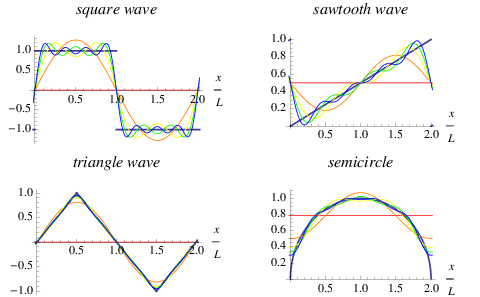
\includegraphics[width=0.5\textwidth]{figures/Fourier_Series.png}
\caption{\label{fig:fourier} The Fourier series representing four different periodic functions.}
\end{figure}
\end{frame}

\section{Complex numbers 1: programming with Octave}

\begin{frame}{Complex numbers 1: programming with Octave}
Let's take the time to get octave installed on your systems: \url{https://www.gnu.org/software/octave}.  \\ \vspace{0.5cm}
If we cannot get it installed on your systems, we can always run it on the local desktops. \\ \vspace{0.5cm}
A good tutorial can be found here: \\
\url{https://en.wikibooks.org/wiki/Octave_Programming_Tutorial}
\end{frame}

\begin{frame}[fragile]{Complex numbers 1: programming with Octave}
Octave is a high-level \textit{scripting} programming language.  Although it is possible to write packages and compile code in octave, the most common application is executing a script that performs some analysis on digital data. \\
\begin{verbatim}
a = 1+1i;
b = conj(a);
a * b
\end{verbatim}
The result of this code should be 2.0.  Why?  We are defining a complex number in the first line, computing the complex conjugate, and multiplying them.
\end{frame}

\begin{frame}[fragile]{Complex numbers 1: programming with Octave}
Octave naturally handles vectors of numbers and matrices.  Let's define a vector of complex numbers. \\
\begin{verbatim}
a = [1 2 3 5 7 11];
size(a)
ans = 1   6
a = a';
size(a)
\end{verbatim}
The code in the fourth line \textit{transposes} the vector.  This means trading the rows for the columns of the vector.  What begins as a $1 \times 6$ vector (one row by six columns) ends as a $6 \times 1$ vector (six rows by one column).
\end{frame}

\begin{frame}[fragile]{Complex numbers 1: programming with Octave}
Operations are as expected, but we need special notation for vectoral calculations:
\begin{verbatim}
a = 2.0;
b = 4.0;
b/a
ans = 2
b = [4.0 4.0 4.0]
b/a
ans =
2   2   2
a./b
ans =
0.5   0.5   0.5
\end{verbatim}
\end{frame}

\begin{frame}[fragile]{Complex numbers 1: programming with Octave}
Placing a dot (.) before a standard operation indicates that the operation is to be carried out in a vectoral-sense.
\begin{verbatim}
t1 = [1 2 3 4 5 6 7 8 9 10];
t2 = t1+1;
t1.*t2
ans =
2   6   12   20   30   42   56   72   90   110
\end{verbatim}
\end{frame}

\begin{frame}[fragile]{Complex numbers 1: programming with Octave}
The colon operator (:) represents iteration in octave.  Consider three cases:  \\
\begin{verbatim}
fs = 1000.0;
t = [0.0:1/fs:10.0];
plot(t,sin(2.0 * pi * 3.0 .* t));
\end{verbatim}
Octave should produce a plot of a sine wave with a frequency of 3.0 Hz (if the time is in seconds).  How can you tell?
\end{frame}

\begin{frame}[fragile]{Complex numbers 1: programming with Octave}
Count the number of complete oscillations in 2.0 seconds.  Do you see 6.0 oscillations?  What is the significance of $f_s$ in the code?
\begin{verbatim}
fs = 1000.0;
t = [0.0:1/fs:10.0];
plot(t,sin(2.0 * pi * 3.0 .* t));
\end{verbatim}
The \alert{axis} command is useful for controlling the plotted region:
\begin{verbatim}
axis([0 2 -2 2]);
\end{verbatim}
\end{frame}

\begin{frame}[fragile]{Complex numbers 1: programming with Octave}
The colon operator (:) also refer to elements in a vector.
\begin{verbatim}
t(1)
ans =
0
t(2:5)
ans = 
0.001   0.002   0.003   0.004
t(:)
ans = 
(should be the whole vector)
t(1:end)
ans =
(should be the whole vector)
\end{verbatim}
\end{frame}

\section{Conclusion}

\begin{frame}{Conclusion}
Text
\end{frame}

\end{document}
